% Options for packages loaded elsewhere
\PassOptionsToPackage{unicode}{hyperref}
\PassOptionsToPackage{hyphens}{url}
%
\documentclass[
  a4paper,
]{scrbook}

\usepackage{amsmath,amssymb}
\usepackage{iftex}
\ifPDFTeX
  \usepackage[T1]{fontenc}
  \usepackage[utf8]{inputenc}
  \usepackage{textcomp} % provide euro and other symbols
\else % if luatex or xetex
  \usepackage{unicode-math}
  \defaultfontfeatures{Scale=MatchLowercase}
  \defaultfontfeatures[\rmfamily]{Ligatures=TeX,Scale=1}
\fi
\usepackage{lmodern}
\ifPDFTeX\else  
    % xetex/luatex font selection
\fi
% Use upquote if available, for straight quotes in verbatim environments
\IfFileExists{upquote.sty}{\usepackage{upquote}}{}
\IfFileExists{microtype.sty}{% use microtype if available
  \usepackage[]{microtype}
  \UseMicrotypeSet[protrusion]{basicmath} % disable protrusion for tt fonts
}{}
\makeatletter
\@ifundefined{KOMAClassName}{% if non-KOMA class
  \IfFileExists{parskip.sty}{%
    \usepackage{parskip}
  }{% else
    \setlength{\parindent}{0pt}
    \setlength{\parskip}{6pt plus 2pt minus 1pt}}
}{% if KOMA class
  \KOMAoptions{parskip=half}}
\makeatother
\usepackage{xcolor}
\setlength{\emergencystretch}{3em} % prevent overfull lines
\setcounter{secnumdepth}{5}
% Make \paragraph and \subparagraph free-standing
\makeatletter
\ifx\paragraph\undefined\else
  \let\oldparagraph\paragraph
  \renewcommand{\paragraph}{
    \@ifstar
      \xxxParagraphStar
      \xxxParagraphNoStar
  }
  \newcommand{\xxxParagraphStar}[1]{\oldparagraph*{#1}\mbox{}}
  \newcommand{\xxxParagraphNoStar}[1]{\oldparagraph{#1}\mbox{}}
\fi
\ifx\subparagraph\undefined\else
  \let\oldsubparagraph\subparagraph
  \renewcommand{\subparagraph}{
    \@ifstar
      \xxxSubParagraphStar
      \xxxSubParagraphNoStar
  }
  \newcommand{\xxxSubParagraphStar}[1]{\oldsubparagraph*{#1}\mbox{}}
  \newcommand{\xxxSubParagraphNoStar}[1]{\oldsubparagraph{#1}\mbox{}}
\fi
\makeatother


\providecommand{\tightlist}{%
  \setlength{\itemsep}{0pt}\setlength{\parskip}{0pt}}\usepackage{longtable,booktabs,array}
\usepackage{calc} % for calculating minipage widths
% Correct order of tables after \paragraph or \subparagraph
\usepackage{etoolbox}
\makeatletter
\patchcmd\longtable{\par}{\if@noskipsec\mbox{}\fi\par}{}{}
\makeatother
% Allow footnotes in longtable head/foot
\IfFileExists{footnotehyper.sty}{\usepackage{footnotehyper}}{\usepackage{footnote}}
\makesavenoteenv{longtable}
\usepackage{graphicx}
\makeatletter
\def\maxwidth{\ifdim\Gin@nat@width>\linewidth\linewidth\else\Gin@nat@width\fi}
\def\maxheight{\ifdim\Gin@nat@height>\textheight\textheight\else\Gin@nat@height\fi}
\makeatother
% Scale images if necessary, so that they will not overflow the page
% margins by default, and it is still possible to overwrite the defaults
% using explicit options in \includegraphics[width, height, ...]{}
\setkeys{Gin}{width=\maxwidth,height=\maxheight,keepaspectratio}
% Set default figure placement to htbp
\makeatletter
\def\fps@figure{htbp}
\makeatother
% definitions for citeproc citations
\NewDocumentCommand\citeproctext{}{}
\NewDocumentCommand\citeproc{mm}{%
  \begingroup\def\citeproctext{#2}\cite{#1}\endgroup}
\makeatletter
 % allow citations to break across lines
 \let\@cite@ofmt\@firstofone
 % avoid brackets around text for \cite:
 \def\@biblabel#1{}
 \def\@cite#1#2{{#1\if@tempswa , #2\fi}}
\makeatother
\newlength{\cslhangindent}
\setlength{\cslhangindent}{1.5em}
\newlength{\csllabelwidth}
\setlength{\csllabelwidth}{3em}
\newenvironment{CSLReferences}[2] % #1 hanging-indent, #2 entry-spacing
 {\begin{list}{}{%
  \setlength{\itemindent}{0pt}
  \setlength{\leftmargin}{0pt}
  \setlength{\parsep}{0pt}
  % turn on hanging indent if param 1 is 1
  \ifodd #1
   \setlength{\leftmargin}{\cslhangindent}
   \setlength{\itemindent}{-1\cslhangindent}
  \fi
  % set entry spacing
  \setlength{\itemsep}{#2\baselineskip}}}
 {\end{list}}
\usepackage{calc}
\newcommand{\CSLBlock}[1]{\hfill\break\parbox[t]{\linewidth}{\strut\ignorespaces#1\strut}}
\newcommand{\CSLLeftMargin}[1]{\parbox[t]{\csllabelwidth}{\strut#1\strut}}
\newcommand{\CSLRightInline}[1]{\parbox[t]{\linewidth - \csllabelwidth}{\strut#1\strut}}
\newcommand{\CSLIndent}[1]{\hspace{\cslhangindent}#1}

\makeatletter
\@ifpackageloaded{tcolorbox}{}{\usepackage[skins,breakable]{tcolorbox}}
\@ifpackageloaded{fontawesome5}{}{\usepackage{fontawesome5}}
\definecolor{quarto-callout-color}{HTML}{909090}
\definecolor{quarto-callout-note-color}{HTML}{0758E5}
\definecolor{quarto-callout-important-color}{HTML}{CC1914}
\definecolor{quarto-callout-warning-color}{HTML}{EB9113}
\definecolor{quarto-callout-tip-color}{HTML}{00A047}
\definecolor{quarto-callout-caution-color}{HTML}{FC5300}
\definecolor{quarto-callout-color-frame}{HTML}{acacac}
\definecolor{quarto-callout-note-color-frame}{HTML}{4582ec}
\definecolor{quarto-callout-important-color-frame}{HTML}{d9534f}
\definecolor{quarto-callout-warning-color-frame}{HTML}{f0ad4e}
\definecolor{quarto-callout-tip-color-frame}{HTML}{02b875}
\definecolor{quarto-callout-caution-color-frame}{HTML}{fd7e14}
\makeatother
\makeatletter
\@ifpackageloaded{caption}{}{\usepackage{caption}}
\AtBeginDocument{%
\ifdefined\contentsname
  \renewcommand*\contentsname{Table of contents}
\else
  \newcommand\contentsname{Table of contents}
\fi
\ifdefined\listfigurename
  \renewcommand*\listfigurename{List of Figures}
\else
  \newcommand\listfigurename{List of Figures}
\fi
\ifdefined\listtablename
  \renewcommand*\listtablename{List of Tables}
\else
  \newcommand\listtablename{List of Tables}
\fi
\ifdefined\figurename
  \renewcommand*\figurename{Figure}
\else
  \newcommand\figurename{Figure}
\fi
\ifdefined\tablename
  \renewcommand*\tablename{Table}
\else
  \newcommand\tablename{Table}
\fi
}
\@ifpackageloaded{float}{}{\usepackage{float}}
\floatstyle{ruled}
\@ifundefined{c@chapter}{\newfloat{codelisting}{h}{lop}}{\newfloat{codelisting}{h}{lop}[chapter]}
\floatname{codelisting}{Listing}
\newcommand*\listoflistings{\listof{codelisting}{List of Listings}}
\makeatother
\makeatletter
\makeatother
\makeatletter
\@ifpackageloaded{caption}{}{\usepackage{caption}}
\@ifpackageloaded{subcaption}{}{\usepackage{subcaption}}
\makeatother

\ifLuaTeX
  \usepackage{selnolig}  % disable illegal ligatures
\fi
\usepackage{bookmark}

\IfFileExists{xurl.sty}{\usepackage{xurl}}{} % add URL line breaks if available
\urlstyle{same} % disable monospaced font for URLs
\hypersetup{
  pdftitle={Many body wavefunctions},
  hidelinks,
  pdfcreator={LaTeX via pandoc}}


\title{Many body wavefunctions}
\author{}
\date{}

\begin{document}
\frontmatter
\maketitle


\mainmatter
\newcommand{\cN}{\mathcal{N}}
\newcommand{\br}{\mathbf{r}}
\newcommand{\bp}{\mathbf{p}}
\newcommand{\bk}{\mathbf{k}}
\newcommand{\bq}{\mathbf{q}}
\newcommand{\bv}{\mathbf{v}}
\newcommand{\brN}{\br_1, \ldots, \br_N}
\newcommand{\xN}{x_1, \ldots, x_N}
\newcommand{\zN}{z_1, \ldots, z_N}
\newcommand{\pop}{\psi^{\vphantom{\dagger}}}
\newcommand{\pdop}{\psi^\dagger}
\newcommand{\Pop}{\Psi^{\vphantom{\dagger}}}
\newcommand{\Pdop}{\Psi^\dagger}
\newcommand{\Phop}{\Phi^{\vphantom{\dagger}}}
\newcommand{\Phdop}{\Phi^\dagger}
\newcommand{\phop}{\phi^{\vphantom{\dagger}}}
\newcommand{\phdop}{\phi^\dagger}
\newcommand{\aop}{a^{\vphantom{\dagger}}}
\newcommand{\adop}{a^\dagger}
\newcommand{\bop}{b^{\vphantom{\dagger}}}
\newcommand{\bdop}{b^\dagger}
\newcommand{\cop}{c^{\vphantom{\dagger}}}
\newcommand{\cdop}{c^\dagger}
\newcommand{\bra}[1]{\langle{#1}\rvert}
\newcommand{\ket}[1]{\lvert{#1}\rangle}
\newcommand{\inner}[2]{\langle{#1}\rvert #2 \rangle}
\newcommand{\braket}[3]{\langle{#1}\rvert #2 \lvert #3 \rangle}
\newcommand{\sgn}{\mathrm{sgn}}
\newcommand{\abs}[1]{\lvert{#1}\rvert}

\[
\DeclareMathOperator{\tr}{tr}
\DeclareMathOperator{\E}{\mathbb{E}}
\]

We begin our study of many body quantum mechanics by examining a number
of systems where eigenstates and eigenvalues may be found explicitly for
any number of particles. Be warned that these situations are
\textbf{highly atypical} -- but are nevertheless very informative.

Reading: (Baym 2018).

\begin{center}\rule{0.5\linewidth}{0.5pt}\end{center}

\chapter{Bosons and Fermions}\label{bosons-and-fermions}

An \(N\) particle quantum system is described by a wavefunction of \(N\)
arguments \(\Psi(\mathbf{r}_1,\ldots, \mathbf{r}_N)\). The starting
point of many body quantum mechanics is that:

\begin{tcolorbox}[enhanced jigsaw, rightrule=.15mm, colback=white, opacityback=0, left=2mm, toprule=.15mm, breakable, leftrule=.75mm, colframe=quarto-callout-warning-color-frame, arc=.35mm, bottomrule=.15mm]

Systems of indistinguishable particles are described by \textbf{totally
symmetric} or \textbf{totally antisymmetric} wavefunctions.

\end{tcolorbox}

Just to be clear, \emph{totally symmetric} means the wavefunction is
unchanged by exchanging any two coordinates, whereas \emph{totally
antisymmetric} means that it changes sign.

A good fraction of this course is devoted to exploring the ramifications
of this fact. Perhaps we should therefore give a \emph{very} quick
summary of why it appears to be true.

The first question is: what \emph{are} indistinguishable particles? I'll
give a theorist's answer. Indistinguishable particles are those
described by Hamiltonians that are invariant under permuting the
particle's labels. Thus the sum of single particle Hamiltonians

\[
H = \sum_{i=1}^{N} \left[-\frac{\nabla_i^{2}}{2m}+V(\mathbf{r_i})\right]
\]

\emph{{[}did you remember that \(\hbar=1\)?{]}} describes
indistinguishable particles while

\[
H = \sum_{i=1}^{N} \left[-\frac{\nabla_i^{2}}{2m_i}+V(\mathbf{r_i})\right]
\]

does not, on account of the masses being all different. Any time we have
a symmetry operation that commutes with the Hamiltonian, the eigenstates
of that symmetry are preserved by time evolution with that Hamiltonian.
Thus a symmetric potential \(V(x)=V(-x)\) commutes with the parity
operation \(x\to -x\), so the eigenstates of this operation -- the even
and odd wavefunctions -- are preserved by time evolution.

The Hamiltonian of indistinguishable particles commutes with every
operator of particle exchange, defined by \[
P_{ij}\Psi(\mathbf{r}_1,\ldots, \mathbf{r}_i,\ldots, \mathbf{r}_j,\ldots \mathbf{r}_N) = \Psi(\mathbf{r}_1,\ldots, \mathbf{r}_j,\ldots, \mathbf{r}_i,\ldots \mathbf{r}_N).
\]

These operators satisfy \(P_{ij}^2=\mathbb{1}\), so their eigenvalues
are \(\pm 1\), corresponding to states that are either symmetric or
antisymmetric under exchange. The only simultaneous eigenstates of all
particle exchange operations (note that different exchanges don't
commute if they involve the same particle) are the totally symmetric and
antisymmetric wavefunctions. Thus these properties are preserved by time
evolution. It's always been this way.

We classify particles into symmetric \textbf{bosons} and antisymmetric
\textbf{fermions}, named for Bose and Fermi respectively (the whimsical
terminology is Dirac's). The distinction works equally well for
composite particles, provide we ignore the internal degrees of freedom
and discuss only the center of mass coordinate.

All matter in the universe is made up of fermions: electrons, quarks,
etc., but you can easily convince yourself that an even number of
fermions make a composite boson (e.g.~a \(^4\)He atom with two
electrons, two neutrons and two protons) and an odd number make a
composite fermion (\(^3\)He has one fewer neutron, which in turn is made
up of 3 quarks).

\section{Two Particles}\label{two-particles}

A pair of particles is described by a wavefunction
\(\Psi(\mathbf{x},\mathbf{y})\). If we are dealing with distinguishable
particles, the wavefunction of a pair of particles in states
\(\lvert{\varphi_1}\rangle\) and \(\lvert{\varphi_2}\rangle\) would be

\begin{equation}\phantomsection\label{eq-product-wavefunction}{
\Psi(\mathbf{r}_1,\mathbf{r}_2)=\varphi_1(\mathbf{r}_1)\varphi_2(\mathbf{r}_2).
}\end{equation}

Accounting for indistinguishability, we have either

\begin{equation}\phantomsection\label{eq-sym}{
\Psi(\mathbf{r}_1,\mathbf{r}_2)=\frac{1}{\sqrt{2}}[\varphi_1(\mathbf{r}_1)\varphi_2(\mathbf{r}_2)\pm \varphi_2(\mathbf{r}_1)\varphi_1(\mathbf{r}_2)]
}\end{equation}

with the upper sign for bosons and the lower for fermions (The
\(1/\sqrt{2}\) yields a normalized wavefunction if
\(\varphi_{1,2}(\mathbf{r})\) are orthonormal.). Note in particular that
when \(\varphi_1=\varphi_2\) the fermion wavefunction \emph{vanishes}.
This illustrates the \textbf{Pauli exclusion principle}, that no two
identical fermions can be in the same quantum state. There is no such
restriction for bosons.

Classically, if you had a function \(\rho_{1}(\mathbf{r}_1)\) describing
the probability density of finding particle \(1\) at position
\(\mathbf{r}_1\), and the corresponding quantity for an independent
particle \(2\), you would have no hesitation in concluding that the
joint distribution is

\[
\rho_{12}(\mathbf{r}_1,\mathbf{r}_2)=\rho_1(\mathbf{r}_1)\rho_2(\mathbf{r}_2).
\label{eq:classicaljoint}
\]

This also follows from taking the square modulus of
Equation~\ref{eq-product-wavefunction}. The result implied by the
wavefunction Equation~\ref{eq-sym} is \[
\begin{align}
\rho_{12}(\mathbf{r}_1,\mathbf{r}_2) &= \frac{1}{2}\left[\rho_1(\mathbf{r}_1)\rho_2(\mathbf{r}_2)+\rho_1(\mathbf{r}_2)\rho_2(\mathbf{r}_1)\right] \\
&\pm\frac{1}{2}\left[\varphi^{}_1(\mathbf{r}_1)\varphi^*_2(\mathbf{r}_1)\varphi^{}_2(\mathbf{r}_2)\varphi^*_1(\mathbf{r}_2)+\varphi^{}_1(\mathbf{r}_2)\varphi^*_2(\mathbf{r}_2)\varphi^{}_2(\mathbf{r}_1)\varphi^*_1(\mathbf{r}_1)\right].
\end{align}
\]

In particular, \(\rho_{12}(\mathbf{r},\mathbf{r}) = 0\) for fermions,
and
\(\rho_{12}(\mathbf{r},\mathbf{r}) = 2\rho_1(\mathbf{r})\rho_2(\mathbf{r})\)
for bosons. The first result is natural from the standpoint of the
exclusion principle, while the second is perhaps more surprising. This
shows that, because probabilities arise from the squares of amplitudes,
identical particles in quantum mechanics are never truly independent.

One dramatic illustration of this deviation from our classical intuition
is provided by the
\href{https://en.wikipedia.org/wiki/Hong\%E2\%80\%93Ou\%E2\%80\%93Mandel_effect}{Hong--Ou--Mandel}
effect in quantum optics. In simplified terms, we imagine wavepackets
describing two photons (bosons) approaching a 50:50 beam splitter from
either side. Because of the unitarity of scattering, the two photons end
up in orthogonal states. For example, \[
\begin{align}
\lvert{\text{Left}}\rangle\to\frac{1}{\sqrt{2}}\left(\lvert{\text{Left}}\rangle+ \lvert{\text{Right}}\rangle\right)\\\\
\lvert{\text{Right}}\rangle\to\frac{1}{\sqrt{2}}\left(\lvert{\text{Left}}\rangle- \lvert{\text{Right}}\rangle\right)
\end{align}
\]

\begin{tcolorbox}[enhanced jigsaw, rightrule=.15mm, opacityback=0, bottomtitle=1mm, colbacktitle=quarto-callout-tip-color!10!white, colback=white, toprule=.15mm, titlerule=0mm, arc=.35mm, title=\textcolor{quarto-callout-tip-color}{\faLightbulb}\hspace{0.5em}{Check}, left=2mm, opacitybacktitle=0.6, breakable, leftrule=.75mm, bottomrule=.15mm, colframe=quarto-callout-tip-color-frame, toptitle=1mm, coltitle=black]

If we start in \[
\frac{1}{\sqrt{2}}[\varphi_\text{L}(\mathbf{r}_1)\varphi_\text{R}(\mathbf{r}_2)\pm \varphi_\text{R}(\mathbf{r}_1)\varphi_\text{L}(\mathbf{r}_2)]
\] What state do we end up in?

\end{tcolorbox}

\begin{figure}[H]

{\centering 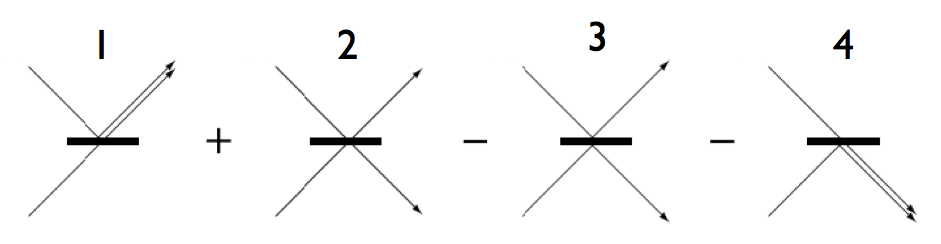
\includegraphics{../assets/HOM.png}

}

\caption{Four possible outcomes after the passage of two bosons through
a beam splitter.}

\end{figure}%

\section{Product States}\label{product-states}

The Hamiltonian of a system of \(N\) identical noninteracting particles
is a sum of \(N\) identical \textbf{single particle} Hamiltonians, that
is, with each term acting on a different particle coordinate

\[
 H = \sum_{i=1}^{N} \left[-\frac{\nabla_i^{2}}{2m}+V(\mathbf{r}_i)\right]
 \label{quantum_statistics_SPHamiltonian}
\]

where \(m\) is the particle mass, and \(V(\mathbf{r})\) is a potential
experienced by the particles.

Let's denote the eigenstates of the single particle Hamiltonian by
\(\{\varphi_\alpha(\mathbf{r})\}\) , and the corresponding eigenenergies
by \(\{E_\alpha\}\), where \(\alpha\) is a shorthand for whatever
quantum numbers are used to label the states.

A set of labels \(\{\alpha_{i}\}\) \(i=1,2,\ldots N\) tells us the state
of each of the particles. Thus we can write an eigenstat\ale of \(N\)
\emph{distinguishable} particles with energy
\(E=\sum_{i=1}^{N}E_{\alpha_{i}}\) as

\begin{equation}\phantomsection\label{eq-distinguishable}{
\lvert{\Psi_{\alpha_{1}\alpha_{2}\cdots \alpha_{N}}}\rangle=\varphi_{\alpha_{1}}(\mathbf{r_{1}})\varphi_{\alpha_{2}}(\mathbf{r_{2}})\cdots\varphi_{\alpha_{N}}(\mathbf{r_{N}})
}\end{equation}

(We will frequently switch between the wavefunction
\(\varphi(\mathbf{x})\) and bra-ket notation \(\lvert{\varphi}\rangle\).
In the latter notation the product wavefunction in
Equation~\ref{eq-product-wavefunction} is written
\(\lvert{\varphi_{1}}\rangle\lvert{\varphi_{2}}\rangle\))

Such states are called \textbf{product states}. A general state will be
expressed as a superposition of product states: they are special states
which provide a frequently convenient basis.

As we've just discussed, however, we should really be dealing with a
totally symmetric or totally antisymmetric wavefunction, depending on
whether our identical particles are bosons or fermions. To write these
down we introduce the operators of \emph{symmetrization} and
\emph{antisymmetrization}

\begin{equation}\phantomsection\label{eq-sym-antisym}{
\mathcal{S}=\frac{1}{N!}\sum_{\pi} P_\pi, \qquad \mathcal{A}=\frac{1}{N!}\sum_{\pi} \mathrm{sgn}(\pi)P_\pi
}\end{equation}

Here's the definition of the various quantities in
Equation~\ref{eq-sym-antisym}:

\begin{itemize}
\tightlist
\item
  The sums are over all \(N!\) permutations \(\pi\) of \(N\) objects.
  One way to think of a permutation \(\pi\) is as a one-to-one
  correspondence (or
  \href{https://en.wikipedia.org/wiki/Bijection}{bijection}) between the
  set \(\{1,2,\ldots N\}\) and itself, so that 1 is mapped to
  \(\pi(1)\), etc..
\item
  \(P_\pi\) denotes the corresponding permutation operator \[
  P_\pi \Psi(\mathbf{r}_1,\mathbf{r}_2,\ldots \mathbf{r}_N) = \Psi(\mathbf{r}_{\pi(1)}, \mathbf{r}_{\pi(2)},\ldots \mathbf{r}_{\pi(N)})
  \]
\item
  \(\mathrm{sgn}(\pi)\) is the
  \href{https://en.wikipedia.org/wiki/Parity_of_a_permutation}{signature}
  of the permutation, equal to \(+1\) for permutations involving an even
  number of exchanges (transpositions), and \(-1\) for an odd number.
  Note that although the same permutation can be accomplished with many
  different sets of transpositions, the number of transpositions is
  either always odd or always even.
\end{itemize}

Equation~\ref{eq-sym-antisym} allows us to write the totally symmetric
and totally antisymmetric versions of Equation~\ref{eq-distinguishable}
as \begin{equation}\phantomsection\label{eq-norm}{
\begin{aligned}
 \lvert{\Psi^{S}_{\alpha_{1}\alpha_{2}\cdots\alpha_{N}}}\rangle&=\sqrt{\frac{N!}{\prod_{\alpha}N_{\alpha}!}}\mathcal{S}\,\varphi_{\alpha_{1}}(\mathbf{r_{1}})\varphi_{\alpha_{2}}(\mathbf{r_{2}})\cdots\varphi_{\alpha_{N}}(\mathbf{r_{N}}) \\
&=\sqrt{\frac{1}{N!\prod_{\alpha}N_{\alpha}!}}\sum_\pi\varphi_{\alpha_{1}}(\mathbf{r_{\pi(1)}})\varphi_{\alpha_{2}}(\mathbf{r_{\pi(2)}})\cdots\varphi_{\alpha_{N}}(\mathbf{r_{\pi(N)}})\\
 \lvert{\Psi^{A}_{\alpha_{1}\alpha_{2}\cdots\alpha_{N}}}\rangle&=\sqrt{N!}\mathcal{A}\,\varphi_{\alpha_{1}}(\mathbf{r_{1}})\varphi_{\alpha_{2}}(\mathbf{r_{2}})\cdots\varphi_{\alpha_{N}}(\mathbf{r_{N}})\\
 &=\sqrt{\frac{1}{N!}}\sum_\pi \mathrm{sgn}(\pi)\varphi_{\alpha_{1}}(\mathbf{r_{\pi(1)}})\varphi_{\alpha_{2}}(\mathbf{r_{\pi(2)}})\cdots\varphi_{\alpha_{N}}(\mathbf{r_{\pi(N)}}),
\end{aligned}
}\end{equation}

where the \textbf{occupation numbers} \(\{N_{\alpha}\}\) in the boson
case give the number of particles in state \(\alpha\). These
normalization factors yield normalized wavefunctions \emph{if} the
single particle state \(\lvert{\varphi_\alpha}\rangle\) are orthonormal
(as the eigenstates of the single particle Hamiltonian are). In the
fermion case each \(N_{\alpha}\) is either \(0\) or \(1\) so the
prefactor simplifies. Since the order of the \(\alpha\) indices is
irrelevant in the boson case, and amounts only to a sign in the fermion
case, states based on a given set of single particle states are more
efficiently labeled by the occupation numbers. In terms of these numbers
the total energy is

\[
 \label{quantum_statistics_TotalEnergy}
 E=\sum_{i=1}^{N}E_{\alpha_{i}}=\sum_{\alpha}N_{\alpha} E_{\alpha}
\]

\begin{tcolorbox}[enhanced jigsaw, rightrule=.15mm, opacityback=0, bottomtitle=1mm, colbacktitle=quarto-callout-tip-color!10!white, colback=white, toprule=.15mm, titlerule=0mm, arc=.35mm, title=\textcolor{quarto-callout-tip-color}{\faLightbulb}\hspace{0.5em}{Check}, left=2mm, opacitybacktitle=0.6, breakable, leftrule=.75mm, bottomrule=.15mm, colframe=quarto-callout-tip-color-frame, toptitle=1mm, coltitle=black]

Verify that the normalization factors in Equation~\ref{eq-norm} are
correct.

\end{tcolorbox}

A more formal way of putting things is as follows. We first consider the
space spanned by states of the form Equation~\ref{eq-distinguishable}.
Then we introduce the operators \(\mathcal{S}\) and \(\mathcal{A}\),
noting that \(\mathcal{S}^{2}=\mathcal{S}\) and
\(\mathcal{A}^{2}=\mathcal{A}\). In other words, there's no point
symmetrizing or antisymmetrizing more than once (we say that the
operators are \textbf{idempotent}). Any eigenvalue of one of these
operators is therefore either one or zero. The states with
\(\mathcal{S}=1\) are the symmetric states, and those with
\(\mathcal{A}=1\) are antisymmetric. You can easily convince yourself
that if a state has one of \(\mathcal{S}\) or \(\mathcal{A}\) equal to
one, the other is zero. This defines symmetric and antisymmetric
subspaces, consisting of the admissible boson and fermion wavefunctions.

Note that the fermion wavefunction takes the form of a \textbf{Slater
determinant} (though it appears first in \{\% cite dirac1926 \%\}).

\begin{equation}\phantomsection\label{eq-slater}{
   \lvert{\Psi^{A}_{\alpha_{1}\alpha_{2}\cdots\alpha_{N}}}\rangle=\frac{1}{\sqrt{N!}}\begin{vmatrix}
   \varphi_{\alpha_{1}}(\mathbf{r_{1}}) &   \varphi_{\alpha_{1}}(\mathbf{r_{2}}) & \cdots & \varphi_{\alpha_{1}}(\mathbf{r_{N}}) \\
   \varphi_{\alpha_{2}}(\mathbf{r_{1}}) &  \cdots & \cdots & \cdots  \\
   \cdots & \cdots & \cdots & \cdots  \\
   \varphi_{\alpha_{N}}(\mathbf{r_{1}}) &  \cdots & \cdots & \varphi_{\alpha_{N}}(\mathbf{r_{N}})
 \end{vmatrix}
}\end{equation}

The vanishing of a determinant when two rows or two columns are
identical means that the wavefunction is zero if two particle
coordinates coincide (\(\mathbf{r}_{i}=\mathbf{r}_{j}\)), or if two
particles occupy the same state (\(\alpha_{i}=\alpha_{j}\)).

\chapter{The 1D Fermi Gas}\label{the-1d-fermi-gas}

Let's consider perhaps the simplest many particle system one can think
of: noninteracting particles on a ring. If the ring has circumference
\(L\), the single particle eigenstates are \[
    \label{quantum_statistics_spstates}
    \varphi_{n}(x)=\frac{1}{\sqrt{L}}\exp\left(ik_n x\right),
\]

with \(k_n=\frac{2\pi n}{L}\), \(n\in\mathbb{Z}\). The corresponding
energies are \(E_{n}=\frac{k_n^2}{2m}\).

\section{Ground State}\label{ground-state}

Let's find the \(N\) particle ground state. For bosons every particle is
in the state \(\lvert{\varphi_{0}}\rangle\) with zero energy:
\(N_{0}=N\). Thus

\[
    \Psi^{S}_0(x_{1},x_{2},\ldots x_{N})=\frac{1}{L^{N/2}}
\]

That was easy! The fermion case is harder.

Since the occupation of each level is at most one, the lowest energy is
obtained by filling each level with one particle, starting at the
bottom. If we have an odd number of particles, this means filling the
levels with \(n=-(N-1)/2, -(N-3)/2,\ldots, -1, 0, 1 \ldots (N-1)/2\)
(for an even number of particles we have to decide whether to put the
last particle at \(n=\pm N/2\)). Introducing the complex variables

\[
z_{i}=\exp(2 \pi i x_{i}/L),
\]

the Slater determinant Equation~\ref{eq-slater} becomes

\begin{equation}\phantomsection\label{eq-1d-det}{
    \Psi^A_0(x_1,\ldots, x_N)=\begin{vmatrix}
    z_{1}^{-(N-1)/2} &  z_{2}^{-(N-1)/2} & \cdots & z_{N}^{-(N-1)/2} \\
    z_{1}^{-(N-3)/2} &  \cdots & \cdots & \cdots  \\
    \cdots & \cdots & \cdots & \cdots  \\
    z_{1}^{(N-1)/2} &  \cdots & \cdots & z_{N}^{(N-1)/2}
\end{vmatrix}.
}\end{equation}

Let's evaluate this complicated looking expression in a simple case.
With three particles we have

\begin{equation}\phantomsection\label{eq-3-particle}{
\begin{align}
    \Psi^A_0(x_1,x_2,x_3)&=\begin{vmatrix}
        z_{1}^{-1} & z_{2}^{-1} & z_{3}^{-1} \\
        1 & 1 & 1 \\
        z_{1} & z_{2} & z_{3}
    \end{vmatrix} = \frac{z_{1}}{z_{2}}-\frac{z_{2}}{z_{1}}+\frac{z_{3}}{z_{1}}-\frac{z_{1}}{z_{3}}+\frac{z_{2}}{z_{3}}-\frac{z_{3}}{z_{2}}\nonumber\\
    &=\left(\sqrt{\frac{z_{3}}{z_{1}}}-\sqrt{\frac{z_{1}}{z_{3}}}\right)\left(\sqrt{\frac{z_{1}}{z_{2}}}-\sqrt{\frac{z_{2}}{z_{1}}}\right)\left(\sqrt{\frac{z_{2}}{z_{3}}}-\sqrt{\frac{z_{3}}{z_{2}}}\right)  \nonumber\\
    &\propto \sin\left(\frac{ \pi[x_{1}-x_{2}]}{L}\right)\sin\left(\frac{ \pi[x_{3}-x_{1}]}{L}\right)\sin\left(\frac{ \pi[x_{2}-x_{3}]}{L}\right)
\end{align} 
}\end{equation}

The vanishing of the wavefunction when \(x_{i}=x_{j}\) is consistent
with the Pauli principle. You should check that additionally it is
periodic and totally antisymmetric.

Equation~\ref{eq-3-particle} generalizes for any (odd) \(N\) so that the
ground state Slater determinant Equation~\ref{eq-1d-det} is proportional
to

\begin{equation}\phantomsection\label{eq-1d-fermi-gs}{
\Psi^A_0(x_1,\ldots, x_N)\propto\prod_{i<j}^{N} \sin\left(\frac{\pi[x_{i}-x_{j}]}{L}\right).
}\end{equation}

\begin{tcolorbox}[enhanced jigsaw, rightrule=.15mm, opacityback=0, bottomtitle=1mm, colbacktitle=quarto-callout-tip-color!10!white, colback=white, toprule=.15mm, titlerule=0mm, arc=.35mm, title=\textcolor{quarto-callout-tip-color}{\faLightbulb}\hspace{0.5em}{Check}, left=2mm, opacitybacktitle=0.6, breakable, leftrule=.75mm, bottomrule=.15mm, colframe=quarto-callout-tip-color-frame, toptitle=1mm, coltitle=black]

Show this using the \textbf{Vandermonde determinant} \[
\begin{vmatrix}
1 & 1 & \cdots & 1 \\
z_{1} &  z_{2} & \cdots & \cdots  \\
z_{1}^{2} & z_{2}^{2} & \cdots & \cdots  \\
z_{1}^{N-1} &  z_{2}^{N-1} & \cdots & z_{N}^{N-1}
\end{vmatrix}=\prod_{i<j}^{N}(z_{j}-z_{i})
\] which can be proved in a variety of ways. Proving directly that
Equation~\ref{eq-1d-fermi-gs} is an eigenstate of the Hamiltonian is not
easy, but can be accomplished using the identity

\[
\begin{equation}
\label{2nd_quant_cotident}
\cot(x-y)\cot(y-z)+\cot(y-z)\cot(z-x)+\cot(z-x)\cot(x-y)=1. \nonumber
\end{equation}
\]

Check carefully that Equation~\ref{eq-1d-fermi-gs} is periodic and
totally antisymmetric.

\end{tcolorbox}

Let's take the opportunity to introduce some terminology. The wavevector
of the last fermion added is called the \textbf{Fermi wavevector} and
denoted \(k_\text{F}\). In this case \(k_\text{F}=\frac{(N-1)\pi}{L}\).
Its energy \(E_{F}=\frac{k_\text{F}^{2}}{2m}\) is the \textbf{Fermi
energy}.

\section{Density; Density Matrix; Pair
Distribution}\label{density-density-matrix-pair-distribution}

Having a many particle wave function is one thing, but what to \emph{do}
with it? Bear in mind that Equation~\ref{eq-1d-fermi-gs} is just about
the simplest fermion state you can imagine, but it's not immediately
clear what it is telling us.

\(\vert\Psi(x_1,\ldots,x_N)\rvert^2\) is the probability distribution of
the positions of the particles. If we were able to take a photograph of
the positions of the particles at an instant in time, this would
correspond to taking a sample from the probability distribution. In
terms of the complex variables \(z_j\), it would look something like
this:

\begin{figure}

\begin{minipage}{0.50\linewidth}

\centering{

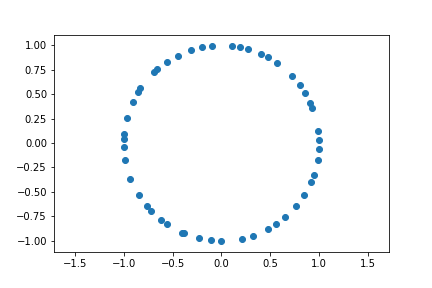
\includegraphics{../assets/1d_fermions.png}

}

\subcaption{\label{fig-fermion}A sample from the probability
distribution \(\lvert\Psi^A_0(z_1,\ldots,z_N)\rvert^2\) for 50
particles.}

\end{minipage}%
%
\begin{minipage}{0.50\linewidth}

\centering{

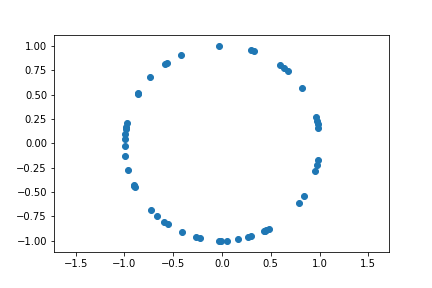
\includegraphics{../assets/poisson_phases.png}

}

\subcaption{\label{fig-poisson}Uniformly distributed points on the
circle described by
\(\vert\Psi^{S}_0(x_{1},x_{2},\ldots x_{N})\rvert^2\). The particle
positions are uncorrelated.}

\end{minipage}%

\caption{\label{fig-1d-dist}Distribution of particle positions for
noninteracting fermion and boson ground states.}

\end{figure}%

Since \(\lvert\Psi(x_1,\ldots,x_N)\rvert^2\) is the probability
distribution of the positions of the particles, we can use it to find
the marginal probability distributions for any subset of the particles.
Of course, since the particles are identical, it doesn't matter which
ones we choose, just the number.

The one particle distribution is related to the average density of
particles, given by
\begin{equation}\phantomsection\label{eq-average-density}{
\rho_1(x_1) = N \int dx_2\ldots dx_N \,\lvert\Psi(x_1,x_2,\ldots,x_N)\rvert^2.
}\end{equation} Note that although I use the symbol \(\rho\), density is
always going to be \emph{number} density (not the mass density).

\begin{tcolorbox}[enhanced jigsaw, rightrule=.15mm, opacityback=0, bottomtitle=1mm, colbacktitle=quarto-callout-tip-color!10!white, colback=white, toprule=.15mm, titlerule=0mm, arc=.35mm, title=\textcolor{quarto-callout-tip-color}{\faLightbulb}\hspace{0.5em}{Check}, left=2mm, opacitybacktitle=0.6, breakable, leftrule=.75mm, bottomrule=.15mm, colframe=quarto-callout-tip-color-frame, toptitle=1mm, coltitle=black]

Can you explain why this is the density? Think about the simpler case of
two particles, with discrete locations. Why is the expected number of
particles at position \(x\) \[
N_x = \sum_y \left[P(x,y) + P(y,x)\right]?
\]

What if we have more particles?

\end{tcolorbox}

Normalization of the wavefunction then implies \[
\int dx\, \rho_1(x) = N.
\] In a translationally invariant system like the fermion gas on a ring
we expect the average density to be constant.

We can regard Equation~\ref{eq-average-density} as an expectation of a
density operator \begin{equation}\phantomsection\label{eq-density-op}{
\rho(x) = \sum_j \delta(x-x_j),
}\end{equation} so that
\(\rho_1(x) = \langle{\Psi}\rvert \rho(x) \lvert \Psi \rangle\).

The \textbf{single particle density matrix} is a generalization of the
expectation of the density, and is defined as (we'll see shortly why
this is a useful quantity)
\begin{equation}\phantomsection\label{eq-spdm}{
g(x,y) \equiv N\int dx_2\ldots dx_N \,\Psi^{}(x,x_2,\ldots,x_N)\Psi^{*}(y,x_2,\ldots,x_N).
}\end{equation} Note that \(g(x,x) = \rho_1(x)\).

\begin{tcolorbox}[enhanced jigsaw, rightrule=.15mm, opacityback=0, bottomtitle=1mm, colbacktitle=quarto-callout-tip-color!10!white, colback=white, toprule=.15mm, titlerule=0mm, arc=.35mm, title=\textcolor{quarto-callout-tip-color}{\faLightbulb}\hspace{0.5em}{Check}, left=2mm, opacitybacktitle=0.6, breakable, leftrule=.75mm, bottomrule=.15mm, colframe=quarto-callout-tip-color-frame, toptitle=1mm, coltitle=black]

Show that the average number of particles in a single particle state
\(\lvert{\psi}\rangle\) is
\begin{equation}\phantomsection\label{eq-nbar}{
\bar N_\psi = \int dx dy\, \psi^*(x)g(x,y)\psi(y).
}\end{equation}

\end{tcolorbox}

\begin{tcolorbox}[enhanced jigsaw, rightrule=.15mm, opacityback=0, bottomtitle=1mm, colbacktitle=quarto-callout-tip-color!10!white, colback=white, toprule=.15mm, titlerule=0mm, arc=.35mm, title=\textcolor{quarto-callout-tip-color}{\faLightbulb}\hspace{0.5em}{Check}, left=2mm, opacitybacktitle=0.6, breakable, leftrule=.75mm, bottomrule=.15mm, colframe=quarto-callout-tip-color-frame, toptitle=1mm, coltitle=black]

Starting from the Slater determinant Equation~\ref{eq-1d-det}
(i.e.~\emph{not} from the explicit form Equation~\ref{eq-1d-fermi-gs}),
show that \(g(x,y)\) for the ground state of the Fermi gas is \[
g(x,y) = \frac{1}{L}\sum_{|k|<k_\text{F}} e^{ik(x-y)} = \int_{k_\text{F}}^{k_\text{F}} \frac{dk}{2\pi} e^{ik(x-y)} = n \frac{\sin \left[k_\text{F}(x-y)\right]}{k_\text{F}(x-y)}
\] where \(n \equiv \frac{k_\text{F}}{\pi}\) is the average density.

\end{tcolorbox}

\begin{tcolorbox}[enhanced jigsaw, rightrule=.15mm, opacityback=0, bottomtitle=1mm, colbacktitle=quarto-callout-tip-color!10!white, colback=white, toprule=.15mm, titlerule=0mm, arc=.35mm, title=\textcolor{quarto-callout-tip-color}{\faLightbulb}\hspace{0.5em}{Check}, left=2mm, opacitybacktitle=0.6, breakable, leftrule=.75mm, bottomrule=.15mm, colframe=quarto-callout-tip-color-frame, toptitle=1mm, coltitle=black]

Find the average number of particles in a momentum state
\(\lvert{k}\rangle\) using Equation~\ref{eq-nbar}
\begin{equation}\phantomsection\label{eq-nk}{
\bar N_k = \begin{cases}
1 & |k|\leq k_\text{F} \\
0 & |k|>k_\text{F}
\end{cases}.
}\end{equation} Note that in a translationally invariant system
\(g(x,y)=g(x-y)\), and is the Fourier transform of \(\bar N_k\).

\end{tcolorbox}

\begin{tcolorbox}[enhanced jigsaw, rightrule=.15mm, opacityback=0, bottomtitle=1mm, colbacktitle=quarto-callout-note-color!10!white, colback=white, toprule=.15mm, titlerule=0mm, arc=.35mm, title=\textcolor{quarto-callout-note-color}{\faInfo}\hspace{0.5em}{Note}, left=2mm, opacitybacktitle=0.6, breakable, leftrule=.75mm, bottomrule=.15mm, colframe=quarto-callout-note-color-frame, toptitle=1mm, coltitle=black]

To understand the origin of the name \emph{single particle density
matrix}, recall that the density matrix \(\varrho\) describes a
\textbf{mixed state} of a quantum system, and is the appropriate
description when the quantum state is not known. \(\varrho\) is a
positive definite hermitian operator satisfying \(\tr \varrho =1\). Its
spectral resolution \[
\varrho = \sum_\alpha p_\alpha \lvert{\varphi_\alpha}\rangle\langle{\varphi_\alpha}\rvert,
\] can be thought of as a statistical mixture of different quantum
states \(\lvert{\varphi_\alpha}\rangle\) with probabilities
\(p_\alpha\).

One natural way in which density matrices arise from pure states is as
follows. The Hilbert space of a composite system consists of a tensor
product of two or more components
\(\mathcal{H}_{AB} = \mathcal{H}_A \otimes \mathcal{H}_B\). Starting
from the density matrix corresponding to a pure state, we can obtain a
density matrix for the component \(A\) alone by `tracing out' the \(B\)
subsystem. \[
\varrho_A = \tr_B \lvert{\Psi}\rangle\langle{\Psi}\rvert,\quad \lvert{\Psi}\rangle\in \mathcal{H}_{AB}.
\] The probability for system \(A\) to be in state
\(\lvert{\psi}\rangle\in \mathcal{H}_A\) is \[
P_\psi = \langle{\psi}\rvert\varrho\lvert{\psi}\rangle.
\] Thus you can think of the single particle density matrix
Equation~\ref{eq-spdm} as arising from tracing out \(N-1\) particles
from an \(N\)-particle system.

We can also consider marginal probability distribution of a pair of
particles, and define the \textbf{pair distribution function} \[
\rho_2(x_1,x_2) = N(N-1) \int dx_3\ldots dx_N \,\left|\Psi(x_1,x_2,\ldots,x_N)\right|^2.
\] The prefactor is to account for all pairs of particles.

\end{tcolorbox}

\begin{tcolorbox}[enhanced jigsaw, rightrule=.15mm, opacityback=0, bottomtitle=1mm, colbacktitle=quarto-callout-tip-color!10!white, colback=white, toprule=.15mm, titlerule=0mm, arc=.35mm, title=\textcolor{quarto-callout-tip-color}{\faLightbulb}\hspace{0.5em}{Check}, left=2mm, opacitybacktitle=0.6, breakable, leftrule=.75mm, bottomrule=.15mm, colframe=quarto-callout-tip-color-frame, toptitle=1mm, coltitle=black]

Starting from the Slater determinant Equation~\ref{eq-1d-det}, show that
\[
\rho_2(x_1,x_2) = n^2\left[1 - \left(\frac{\sin\left[k_\text{F}(x_1-x_2)\right]}{k_\text{F}(x_1-x_2)}\right)^2\right].
\] This vanishes at \(x_1=x_2\), consistent with the Pauli principle.

\end{tcolorbox}

A natural question: \[
\rho_2(x_1,x_2) \overset{?}{=} \langle{\Psi}\rvert\rho(x_1)\rho(x_2)\lvert{\Psi}\rangle.
\] \emph{Almost}. Looking back at Equation~\ref{eq-density-op}, we see
that the product of two density operators will contain terms involving
the same particle, which are absent from \(\rho_2(x_1,x_2)\).

\begin{tcolorbox}[enhanced jigsaw, rightrule=.15mm, opacityback=0, bottomtitle=1mm, colbacktitle=quarto-callout-tip-color!10!white, colback=white, toprule=.15mm, titlerule=0mm, arc=.35mm, title=\textcolor{quarto-callout-tip-color}{\faLightbulb}\hspace{0.5em}{Check}, left=2mm, opacitybacktitle=0.6, breakable, leftrule=.75mm, bottomrule=.15mm, colframe=quarto-callout-tip-color-frame, toptitle=1mm, coltitle=black]

Show that the correct relationship is \[
\rho_2(x_1,x_2) = \langle{\Psi}\rvert\rho(x_1)\rho(x_2)\lvert{\Psi}\rangle - \rho_1(x_1)\delta(x_1-x_2).
\]

\end{tcolorbox}

\section{Impenetrable Bose Gas}\label{impenetrable-bose-gas}

There's a bit more mileage in the 1D Fermi gas yet. Consider the
following Hamiltonian \[
H = -\frac{1}{2m}\sum_j \frac{\partial^2}{\partial x_j^2} + \overbrace{c\sum_{j<k}\delta(x_j-x_k)}^{\equiv H_\text{int}}.
\label{many_LL}
\] The second term represents an interaction between pairs of particles.
Of course, this model is rather special, as (1) it's 1D and (2) the
interaction potential is a \(\delta\)-function. Nevertheless, it
represents a huge step up in difficulty from the noninteracting examples
we've discussed so far. At least, it does for bosons. For fermions, the
wavefunctions vanish at coincident points, and so the interaction has no
effect at all!

For bosons, it happens that the Hamiltonian can still be solved exactly.
For now, however, we'll concern ourselves only with the limit of
infinite interaction: \(c\to \infty\), sometimes called the impenetrable
limit. In this case, \emph{the eigenenergies coincide with those of the
free fermion problem, and the eigenstates are just the modulus of the
corresponding fermion eigenstate}.

\begin{tcolorbox}[enhanced jigsaw, rightrule=.15mm, opacityback=0, bottomtitle=1mm, colbacktitle=quarto-callout-tip-color!10!white, colback=white, toprule=.15mm, titlerule=0mm, arc=.35mm, title=\textcolor{quarto-callout-tip-color}{\faLightbulb}\hspace{0.5em}{Check}, left=2mm, opacitybacktitle=0.6, breakable, leftrule=.75mm, bottomrule=.15mm, colframe=quarto-callout-tip-color-frame, toptitle=1mm, coltitle=black]

Why?

\end{tcolorbox}

Just like that, we've solved our first interacting many body system (and
with infinite coupling, no less)!

Thus the ground state on the ring has the form \[
\Psi_0(x_1,\ldots, x_N) = \prod_{i<j}^{N} \left|\sin\left(\frac{\pi[x_{i}-x_{j}]}{L}\right)\right|.
\]

It's not hard to see why this works. For a state to have a finite
energy, the wavefunction must vanish whenever two coordinates coincide.
This is because the interation energy has the expectation value \[
\langle{\Psi}\rvert H_\text{int} \lvert \Psi \rangle=cN(N-1)\int dx_1\cdots dx_{N-1}\left|
\Psi(x_1,x_1,x_2,\ldots,x_N\right|^2
\] But we already have a complete set of eigenstates that obey this
condition, namely the free fermion Slater determinants. It remains to
make them symmetric functions by taking the modulus.

This mapping is quite powerful, and allows us to calculate any
observable of the impenetrable Bose gas in terms of free fermions
\emph{as long} as that observable is insensitive to taking the modulus
of the wavefunction. Thus the average density \(\rho_1(x)\) and pair
distribution \(\rho_2(x_1,x_2)\) of the previous section can be found in
this way, but the single particle density matrix \(g(x,y)\) cannot.

\begin{tcolorbox}[enhanced jigsaw, rightrule=.15mm, opacityback=0, bottomtitle=1mm, colbacktitle=quarto-callout-tip-color!10!white, colback=white, toprule=.15mm, titlerule=0mm, arc=.35mm, title=\textcolor{quarto-callout-tip-color}{\faLightbulb}\hspace{0.5em}{Check}, left=2mm, opacitybacktitle=0.6, breakable, leftrule=.75mm, bottomrule=.15mm, colframe=quarto-callout-tip-color-frame, toptitle=1mm, coltitle=black]

Show this explicitly.

\end{tcolorbox}

This means that the momentum distribution is \emph{not} given by
Equation~\ref{eq-nk}. Finding \(g(x,y)\) for the impenetrable Bose gas
is in fact really hard. We'll see in a later lecture how to obtain some
of its important features.

\phantomsection\label{refs}
\begin{CSLReferences}{1}{0}
\bibitem[\citeproctext]{ref-baym2018lectures}
Baym, Gordon. 2018. \emph{Lectures on Quantum Mechanics}. CRC Press.

\end{CSLReferences}


\backmatter


\end{document}
